\section{Numerical Experiments}

We implemented the algorithm in C++ language and used the PETSc
\cite{petsc,petsc-efficient,PETSc-user-ref}
package for linear algebra support.
Using a set a benchmark problems we compared its performance
to the limited memory variable metric method L-BFGS-B\cite{Byrd:1995:LMA}.
The calculations were performed using a Pentium II processor with 
512 KB cache and a clock speed of 400MHz and the Linux operating system.


The L-BFGS-B solver also uses a limited memory BFGS matrix to compute
step directions.  However, it does not use projected gradients to update the
matrix.  Instead it updates the full matrix using gradients and
works with reduced matrices $Z^T H Z$ and reduced gradients $Z^T \nabla f$
to compute a step direction.
There process is similar, but not identical
to the procedure used in Example 2.
While BLMVM always works with the full space, L-BFGS-B explicitly
minimizes the function over a sequence of subspaces.
The L-BFGS-B method also uses the compact form of the L-BFGS matrix instead
of the two-loop recursion.

\comment{These differences make the implementation of L-BFGS-B more difficult
that an implementation of BLMVM.
}

\comment{
Computing a step direction in the space of free variables is an unconstrained
optimization problem where a variety of techniques can be applied.
While L-BFGS-B uses the variable metric method in this subspace, 
TRON\cite{lin_c3} applies Newton's method with a trust region
to the space of free variables.  This algorithm enjoys a proof of
convergence and fast local convergence, but it also requires second
derivatives which can be impractical to compute.
}

\begin{table}[bhpt]
\begin{center}
\footnotesize
\begin{tabular}{|l|c|r|rr|rr|c|r|rr|rr|}
\hline
\multicolumn{1}{|c|}{} &
\multicolumn{1}{|c|}{} &
\multicolumn{1}{|c|}{} &
\multicolumn{2}{c|}{BLMVM} &
\multicolumn{2}{c|}{L-BFGS-B} &
\multicolumn{1}{|c|}{} &
\multicolumn{1}{|c|}{} &
\multicolumn{2}{c|}{BLMVM} &
\multicolumn{2}{c|}{L-BFGS-B} \\

\multicolumn{1}{|c|}{Problem}&
\multicolumn{1}{c|}{}&
\multicolumn{1}{c|}{n}&
\multicolumn{1}{c}{nfg}&
\multicolumn{1}{c|}{s}&
\multicolumn{1}{c}{nfg} &
\multicolumn{1}{c|}{s} &
\multicolumn{1}{c|}{}&
\multicolumn{1}{c|}{n}&
\multicolumn{1}{c}{nfg}&
\multicolumn{1}{c|}{s}&
\multicolumn{1}{c}{nfg} &
\multicolumn{1}{c|}{s} \\
\hline
DEPT\_1 & & 2500 &  236 & 1.60 &  235 &  3.02  &   & 10000 &  501 & 14.98 &  502 &  31.61  \\ 
DEPT\_2 & & 2500 &  187 & 1.21 &  179 &  1.93  &   & 10000 &  324 & 9.29 &  420 &  22.49  \\ 
DEPT\_3 & & 2500 &  92 & 0.56 &  93 &  0.78  &   & 10000 &  184 & 5.05 &  233 &  9.49  \\ 
DPJB\_1 & & 2500 &  373 & 2.48 &  10000 &  39.34  &   & 10000 &  690 & 19.76 &  1924 &  107.68  \\ 
DPJB\_2 & & 2500 &  505 & 3.14 &  520 &  5.21  &   & 10000 &  1085 & 29.70 &  1104 &  52.83  \\ 
DPJB\_3 & & 2500 &  2342 & 14.01 &  2607 &  24.68  &   & 10000 &  5680 & 155.11 &  6743 &  307.47  \\ 
DMSA\_A & & 2500 &  307 & 2.99 &  313 &  5.05  &   & 10000 &  680 & 27.40 &  656 &  49.30  \\ 
DMSA\_B & & 2500 &  378 & 3.69 &  552 &  8.84  &   & 10000 &  770 & 31.38 &  1769 &  131.72  \\ 
DMSA\_C & & 2500 &  399 & 3.87 &  942 &  14.71  &   & 10000 &  854 & 34.60 &  2742 &  199.53  \\ 
DMSO\_A & & 2500 &  388 & 3.50 &  390 &  5.99  &   & 10000 &  808 & 31.70 &  749 &  55.25  \\ 
DMSO\_B & & 2500 &  256 & 2.28 &  262 &  4.02  &   & 10000 &  517 & 20.01 &  493 &  36.18  \\ 
DMSO\_C & & 2500 &  340 & 2.69 &  358 &  4.51  &   & 10000 &  777 & 30.31 &  1400 &  102.19  \\ 
DODC\_A & & 2500 &  277 & 2.92 &  260 &  4.38  &   & 10000 &  495 & 22.08 &  499 &  40.18  \\ 
DODC\_B & & 2500 &  218 & 2.33 &  227 &  3.92  &   & 10000 &  471 & 21.53 &  453 &  36.72  \\ 
DODC\_C & & 2500 &  253 & 2.54 &  224 &  3.72  &   & 10000 &  493 & 21.29 &  496 &  38.87  \\ 
DSSC\_A & & 2500 &  172 & 2.95 &  180 &  4.22  &   & 10000 &  345 & 24.48 &  415 &  43.69  \\ 
DSSC\_B & & 2500 &  122 & 2.04 &  139 &  2.97  &   & 10000 &  269 & 18.61 &  275 &  26.44  \\ 
DSSC\_C & & 2500 &  90 & 1.45 &  92 &  1.81  &   & 10000 &  196 & 13.15 &  157 &  13.45  \\ 
DGL1\_A & & 2500 &  10000 & 45.81 &  10000 &  111.05  &   & 10000 &  10000 & 212.65 &  10000 &  564.22  \\ 
DGL1\_B & & 2500 &  10000 & 45.99 &  10000 &  111.02  &   & 10000 &  10000 & 212.89 &  10000 &  565.45  \\ 
DGL2\_A & & 2500 &  1853 & 23.47 &  1643 &  31.52  &   & 10000 &  3172 & 168.77 &  3431 &  301.45  \\ 
DGL2\_B & & 2500 &  3147 & 39.39 &  2969 &  56.70  &   & 10000 &  6490 & 348.66 &  6109 &  542.75  \\ 
DGL2\_C & & 2500 &  5342 & 67.40 &  5561 &  106.08  &   & 10000 &  10000 & 537.10 &  10000 &  883.52  \\ 

\hline
\end{tabular}
\caption{Performance on MINPACK-2 Problems.}
\label{minpack2}
\end{center}
\end{table}

\comment{
We have tested our limited memory variable metric method for bound constrained
optimization on problems
and compared the results with L-BFGS-B.  
}

Table \ref{minpack2} shows the performance of each solver on
bound constrained optimization problems in the MINPACK-2\cite{minpack2test} 
test suite.
Table \ref{minpacksys} shows the performance solving systems of
nonlinear equations in the MINPACK-2 test suite.  We minimized the
square of the Euclidean norm of the residual.  The variables in these
problems are not constrained by bounds.
Table \ref{cute} shows the peformance of the solvers for bound constrained
problems in the CUTE test suite.
On the optimization problems,
both codes
were terminated when
\[ \| \tcc \nabla f(x_k) \| \leq  \mbox{min}\{ 10^{-5}, 10^{-10} |f(x_k)| \}. \]
For the nonlinear equations, the solvers were terminated when
the objective function was less the $10^{-4}$.
These tables show the time  and the number of 
function evaluations required to solve each problem.
With each function evaluation, the solvers also received the gradient.
We limited the solvers to $10,000$ function and gradient evaluations 
per problem.   Problems requiring less than $0.03$ seconds to solve were not
included in the test suite.


\begin{table}[bhpt]
\begin{center}
\footnotesize
\begin{tabular}{|lrr|rr|rr|}
\hline
\multicolumn{3}{|c|}{} &
\multicolumn{2}{c|}{BLMVM} &
\multicolumn{2}{c|}{L-BFGS-B} \\

\multicolumn{1}{|c}{Problem}&
\multicolumn{1}{c}{}&
\multicolumn{1}{c|}{n}&
\multicolumn{1}{c}{nfg}&
\multicolumn{1}{c|}{seconds}&
\multicolumn{1}{c}{nfg} &
\multicolumn{1}{c|}{seconds} \\
\hline
DSFD & & 140 &  251 & 1.24 &  234 &  1.43  \\ 
DSFD & & 350 &  393 & 3.86 &  358 &  4.63  \\ 
DSFD & & 700 &  592 & 10.71 &  645 &  15.86  \\ 
DSFD & & 1400 &  1189 & 41.69 &  1206 &  57.24  \\ 
DFIC & & 80 &  835 & 2.15 &  941 &  3.04  \\ 
DFIC & & 200 &  1890 & 8.89 &  2289 &  14.23  \\ 
DFIC & & 400 &  5444 & 45.33 &  4411 &  49.71  \\ 
DFIC & & 800 &  9970 & 155.20 &  8168 &  174.55  \\ 
DSFI & & 100 &  49 & 0.04 &  45 &  0.07  \\ 
DSFI & & 625 &  121 & 0.57 &  128 &  1.24  \\ 
DSFI & & 2500 &  437 & 8.45 &  416 &  16.52  \\ 
DSFI & & 10000 &  1451 & 125.04 &  1527 &  281.68  \\ 
DFDC & & 100 &  502 & 5.53 &  621 &  7.28  \\ 
DFDC & & 625 &  586 & 44.83 &  618 &  49.73  \\ 
DFDC & & 2500 &  587 & 195.95 &  595 &  206.08  \\ 
DFDC & & 10000 &  355 & 502.35 &  353 &  526.91  \\ 
\hline
\end{tabular}
\caption{Performance Solving Nonlinear Equations.}
\label{minpacksys}
\end{center}
\end{table}




\begin{table}[bhpt]
\begin{center}
\footnotesize
\begin{tabular}{|lr|rr|rr|}
\hline
\multicolumn{2}{|c|}{} &
\multicolumn{2}{c|}{BLMVM} &
\multicolumn{2}{c|}{L-BFGS-B} \\

\multicolumn{1}{|c}{Problem}&
\multicolumn{1}{c|}{n}&
\multicolumn{1}{c}{nfg}&
\multicolumn{1}{c|}{seconds}&
\multicolumn{1}{c}{nfg} &
\multicolumn{1}{c|}{seconds} \\
\hline
BDEXP &  5000 &  20 & 0.42 &        20 &  0.68  \\ 
BIGGSB1 &  1000 &  1574 & 2.77 &        2847 &  12.15  \\ 
CHENHARK &  1000 &  10000 & 19.04 &        9686 &  36.82  \\ 
EXPLIN &  1000 &  67 & 0.06 &        36 &  0.05  \\ 
EXPLIN2 &  1000 &  29 & 0.03 &        23 &  0.03  \\ 
EXPQUAD &  1000 &  179 & 0.26 &        71 &  0.29  \\ 
GRIDGENA &  578 &  61 & 0.13 &        10000 &  24.57  \\ 
HADAMALS &  1024 &  32 & 0.63 &        24 &  0.47  \\ 
HARKERP2 &  1000 &  75 & 6.43 &        10000 &  855.74  \\ 
JNLBRNG1 &  15625 &  466 & 48.43 &        10000 &  929.87  \\ 
JNLBRNG2 &  15625 &  714 & 74.78 &        752 &  108.28  \\ 
JNLBRNGA &  15625 &  435 & 40.24 &        403 &  53.13  \\ 
JNLBRNGB &  15625 &  2377 & 221.85 &        2748 &  355.67  \\ 
LINVERSE &  1999 &  824 & 10.76 &        742 &  12.56  \\ 
MCCORMCK &  10000 &  16 & 0.79 &        15 &  1.18  \\ 
NCVXBQP1 &  10000 &  2 & 0.06 &        2 &  0.07  \\ 
NCVXBQP2 &  10000 &  132 & 3.09 &        10000 &  174.06  \\ 
NCVXBQP3 &  10000 &  124 & 3.41 &        10000 &  171.98  \\ 
NOBNDTOR &  14884 &  310 & 28.10 &        343 &  46.70  \\ 
NONSCOMP &  10000 &  51 & 1.67 &        55 &  3.65  \\ 
OBSTCLAE &  15625 &  233 & 21.84 &        701 &  100.17  \\ 
OBSTCLAL &  15625 &  168 & 15.76 &        197 &  24.88  \\ 
OBSTCLBL &  15625 &  143 & 13.35 &        382 &  55.39  \\ 
OBSTCLBM &  15625 &  166 & 15.66 &        185 &  26.43  \\ 
OBSTCLBU &  15625 &  152 & 14.23 &        227 &  32.12  \\ 
QR3DLS &  610 &  10000 & 75.73 &        10000 &  91.11  \\ 
QRTQUAD &  1000 &  286 & 0.42 &        131 &  0.50  \\ 
SINEALI &  1000 &  65 & 0.16 &        31 &  0.14  \\ 
TORSION1 &  14884 &  222 & 20.10 &        298 &  37.93  \\ 
TORSION2 &  14884 &  272 & 24.63 &        521 &  71.46  \\ 
TORSION3 &  14884 &  123 & 10.98 &        125 &  13.80  \\ 
TORSION4 &  14884 &  122 & 10.77 &        450 &  55.41  \\ 
TORSION5 &  14884 &  63 & 5.65 &        61 &  6.15  \\ 
TORSION6 &  14884 &  75 & 6.60 &        342 &  40.23  \\ 
TORSIONA &  14884 &  241 & 24.88 &        299 &  41.82  \\ 
TORSIONB &  14884 &  278 & 28.70 &        449 &  67.39  \\ 
TORSIONC &  14884 &  133 & 13.78 &        130 &  16.22  \\ 
TORSIOND &  14884 &  129 & 13.34 &        450 &  60.70  \\ 
TORSIONE &  14884 &  62 & 6.34 &        52 &  5.88  \\ 
TORSIONF &  14884 &  75 & 7.58 &        338 &  43.71  \\ 

\hline
\end{tabular}
\caption{Performance on CUTE Problems.}
\label{cute}
\end{center}
\end{table}

\begin{figure}[ht]
\begin{center}
\caption{Comparson of BLMVM and L-BFGS-B.}
   \subfigure[Time]{
   \label{PT}
   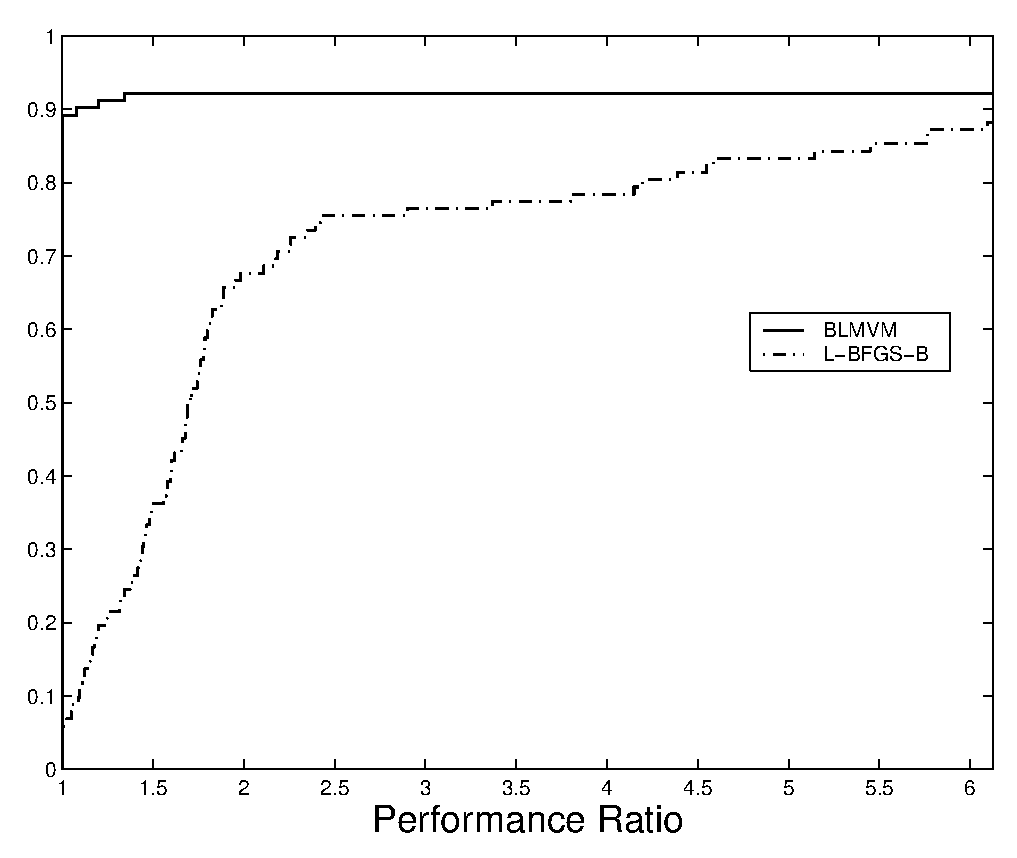
\includegraphics[width=0.45\textwidth,height=0.4\textwidth]{h1.eps}}
   \hskip 0.00\textwidth
   \subfigure[Function Evaluations]{
   \label{PFG}
   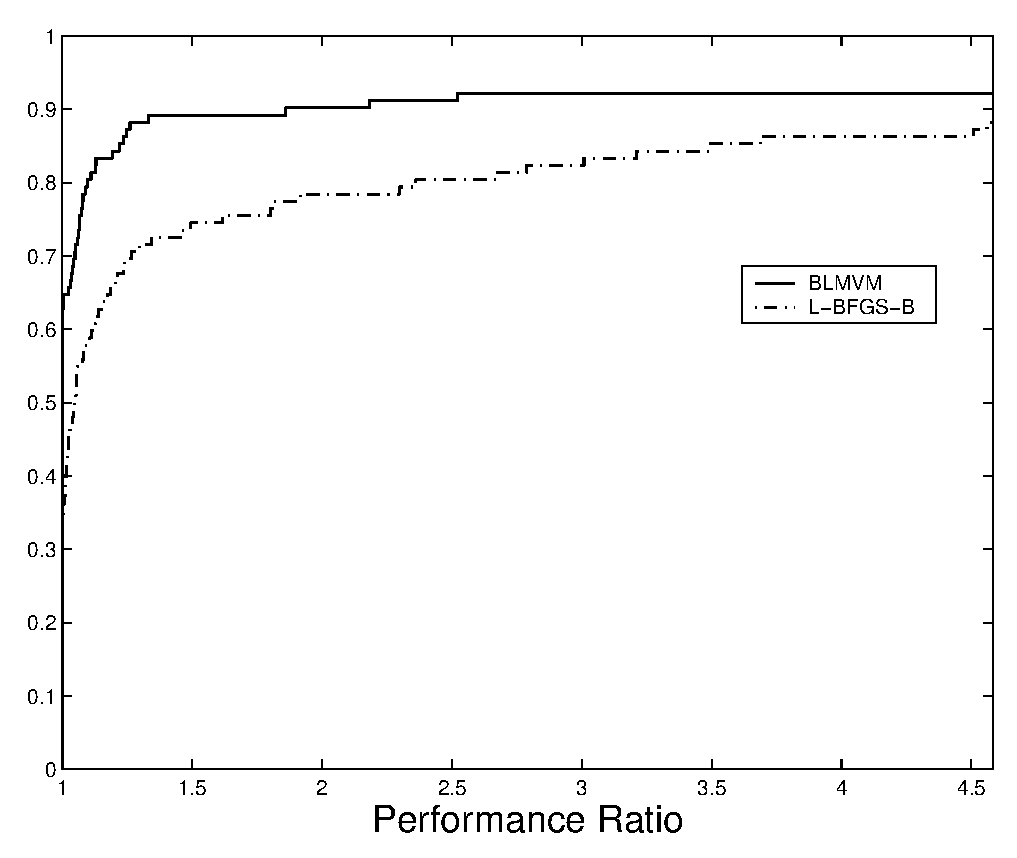
\includegraphics[width=0.45\textwidth,height=0.4\textwidth]{h2.eps}} \\
\label{figure3}
\end{center}
\end{figure}

We applied the performance profiling techniques introduced by Dolan
and Mor\'e\cite{dolan2} to
interpret the results.
Their profiles require a single statistic that measures the performance
of a solver on a problem.  We computed one profile using execution time
and another using the number of function and gradient evaluations.

To create these performance profiles, we first identify the best solver
for each  problem in the test suite.  
Then we compute the ratio of each solver's performance
versus the performance of the best solver.  A ratio of $1.0$ indicates
that the solver was at least as good as the other solvers on that problem
while a ratio greater than one indicates how much worse the solver performed
compared to the best solver.  
When a solver failed to find a solution satisfying the 
specified criteria, we set the ratio to $+\infty$.

Given these ratios, we define a function for each solver.  For every
number greater than or equal to one, this function is
defined to be the percentage of instances where the solver's performance
ratio is less than this number.  This cumulative distribution function
can be plotted for each solver.
The left side of the graph shows how often each solver was the best solver
and the right side of the graph show how often each solver successfully
found a solution.

Figures \ref{figure3} compare the performance of BLMVM to L-BFGS-B
using execution time and number of function evaluations. In both
algorithms, the function and gradient vector were evaluated in
the same routine.
The right side of each graph indicates the robustness of each algorithm
by the percentage of problems that
each algorithm successfully solved.  
Both algorithms fared well by solving about %90/%$ of
the problems to the prescribed accuracy.  BLMVM failed on 8 problems
while L-BFGS-B failed on 12 problems.

The left side of the graphs show the percentage of instances in which each
algorithm performed better than the other.  In terms of function
evaluations, BLMVM used fewer evaluations on about $60\%$ of the problems
while L-BFGS-B used fewer function evaluations on about $30\%$ of the problems.
In terms of execution time, BLMVM performed better on $90\%$ of the test suite,
while  L-BFGS-B used less time on only a few problems.

In addition, we found that when function evaluations were used a measure,
BLMVM performed L-BFGS-B by a factor of two on $15\%$ of the problems and
a factor of three on $10\%$ of the problems.   When execution time was used
as the measure, BLMVM performed L-BFGS-B by a factor of two on $25\%$ of the problems and
a factor of three on $15\%$ of the problems.
On average, BLMVM was about $40\%$ faster than
the competition.  

Since BLMVM uses fewer function evaluations on most problems, we feel that the
step direction used in BLMVM is better than the one used by  L-BFGS-B.  
In terms of execution time, BLMVM shows a
distinct advantage.  In all but a few cases, it found a solution
in less time.  These facts indicate that one iteration of the
BLMVM algorithm is usually cheaper that one iteration of L-BFGS-B.
Whereas L-BFGS-B first identifies a face in the feasible region and
then minimizes over that face, BLMVM always computes a step direction
in the full space.  By not explicitly working in a subspace,
BLMVM saves the time that other algorithms spend identifying it.
These features, and the use of the two-loop recursion instead of the compact
form, make the BLMVM algorithm efficient and relatively simple to implement.

\comment{
The fact that the number of evaluations is less indicates that our
step directions are better.  Even though the theorem only applies
to the when the iterates are on the optimal face, we are gradually
eliminating the effects of the gradient in the free variables.
}

